\chapter{Methodology}
\label{ch:methodology}

\section{Environment and Model}
\label{sec:env_model}
    \subsection{The Procgen Heist Environment}
    \label{subsec:heist_env}
    The Procgen Heist environment, from the suite of procedurally generated environments by \citet{cobbe_2020_leveraging}, was chosen for this research. The agent's objective is to navigate a maze to collect a gem, which may require first collecting up to three keys (in the fixed order of blue, green, red) to open corresponding locks. The environment's procedural generation varies the maze layout and the number of key-lock pairs present in each episode, from zero to three.

    This environment provides a sparse reward signal, with a reward of +10 for reaching the gem and 0 otherwise. This design, coupled with the variable difficulty, establishes a natural curriculum that allows agents to succeed with random exploration in simpler levels before developing a more sophisticated policy.

    The choice of a Procgen environment is motivated by the need to learn generalizable representations. The procedural nature of the mazes discourages the agent from memorizing simple heuristics and instead promotes the development of robust internal models of entities and game mechanics. Furthermore, Heist's multi-objective nature is expected to produce complex internal behaviors, such as general-purpose navigation circuits that can be dynamically retargeted based on the current goal.

    For this investigation, the `easy' distribution of the environment was used, which provides the full 64x64 observation to the agent, making the environment a fully-observable Markov Decision Process (MDP). While memory-based, partially-observable variants exist, they were not used. The distribution of entities is noteworthy: since levels are sampled uniformly from all configurations, the gem and the blue key/lock appear more frequently than the green and red pairs.

    \subsection{Model Architecture}
    \label{subsec:model_arch}
    We train a compressed version of the Impala model that uses 5 convolutional layers instead of 15 as used in the original Impala paper. This architecture comes from~\cite{hilton_2020_understanding} where they find that this model was more interpretable with no discernible loss in performance. We include the model architecture in full in Appendix~\ref{app:model_architecture}.

    When training our model we use a simple PPO implementation from an open source implementation designed to train Procgen models called Procgen-pfrl. We used the easy distribution of the environment due to compute limitations. We tested model training over a number of different batch sizes and distributions. The model checkpoints used to derive our main findings were trained with standard hyperparameters: learning rate 5e-4, 64 parallel environments collecting 256 steps each (16,384 total steps per update), processed in batches of 8 over 3 epochs for 800 million steps. The training dynamics were significantly impacted by changes to batch size often completely collapsing training performance, but over the course of 5 runs with separate seeds with the parameters above we were able to replicate similar model dynamics in each case. 
    \subsection{Model Training}
    \label{subsec:model_training}
    The policy models were trained using Proximal Policy Optimization (PPO) with an open-source implementation based on PFRL, specifically designed for Procgen environments. We also made use of Envpool to accelerate the speed of our training while keeping the actual training dynamics unchanged\cite{weng2022envpool}. Training was conducted until convergence, which in this case was when no statistical improvement was observed for 10000 update steps. The primary model was trained for approximately 600 million steps. 

    To explore the effects of training dynamics on the final learned representations, experiments were run with different training configurations. These variations primarily involved altering the batch geometry through four main hyperparameters: the number of parallel environments, the number of steps per rollout, the mini-batch size, and the number of epochs.


    In the primary configuration reported in this thesis, we used a setup of ($N_{\text{env}}=64$, $N_{\text{step}}=256$, $\texttt{batch\_size}=8$, $n_{\text{epoch}}=3$). In this geometry, the rollout buffer contains $N_{\text{env}}N_{\text{step}}=16\,384$ transitions. This is reshaped into $8$ mini-batches, each containing $B_{\text{mb}}=2\,048$ samples. The optimizer performs $8\times 3 = 24$ gradient steps per PPO update, processing a total of $16\,384\times 3 = 49\,152$ sample-updates per cycle. This configuration was chosen to balance stable learning from large batches with reasonable training time per update.

    We ran 5 sets of training runs for this geometry in order to confirm the repeatability of our results, and ran further training runs with other geometries to observe the extent to which this altered  the final structure of the model weights. Namely ($N_{\text{env}}=128$, $N_{\text{step}}=128$, $\texttt{batch\_size}=8$), ($N_{\text{env}}=256$, $N_{\text{step}}=256$, $\texttt{batch\_size}=8$), and ($N_{\text{env}}=256$, $N_{\text{step}}=128$, $\texttt{batch\_size}=16$). These variants were included to probe the sensitivity of the learned representations to rollout length and batch composition. A detailed comparison of the models trained under these settings is provided in Chapter~\ref{ch:results}.

\section{Interpretability Techniques Employed}
\label{sec:interp_techniques}

\subsection{Feature Visualization}
    \label{subsec:feature_viz}
    A useful initial approach involved simply creating direct visualiations of the convolutional layers of the model. This involved simply taking a given layer and applying a colour spectrum according to the strength of the activations within that region of the grid. This approach, following~\cite{mini_2023_understanding}, provided a direct view of which spatial regions triggered strong positive or negative responses in different channels. Figure~\ref{fig:filter_visualizations} shows an example of this visualization technique applied to multiple layers.


    \begin{figure}[ht]
        \centering
        \begin{tabular}{cccc}
        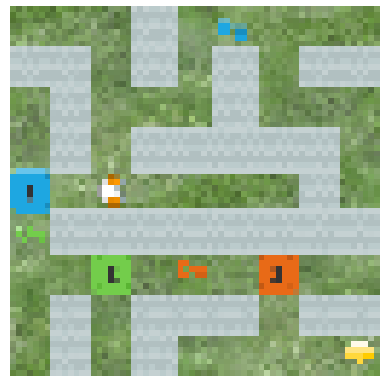
\includegraphics[width=0.25\linewidth]{figures/observation.png}&
        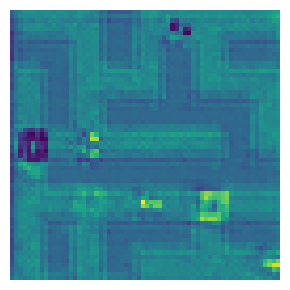
\includegraphics[width=0.25\linewidth]{figures/layer1_filter10.png}&
        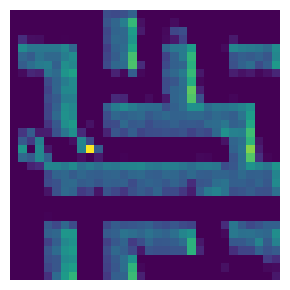
\includegraphics[width=0.25\linewidth]{figures/layer2_filter10.png}&
        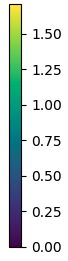
\includegraphics[width=0.067\linewidth]{figures/colorbar.png}
        \end{tabular}
        
        \vspace{0.5em}
        
        \begin{tabular}{ccc}
        \hspace{0.1725\linewidth}&
        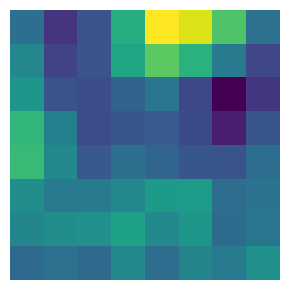
\includegraphics[width=0.25\linewidth]{figures/filter29_layer8_no_title.png}&
        
\includegraphics[width=0.25\linewidth]{figures/filter29_layer9_no_title.png}
        \end{tabular}
        
        \caption{Visualization of the maze and neural network activations in different layers. Top row (left to right): 
        observation input, layer 1 channel 10, layer 2 channel 10, and activation colorbar. 
        Bottom row: layer 8 channel 29 and layer 9 channel 29. In the top row filters we observe a minimal activation around the regions of the blue key and lock and in the bottom row we see maximal activations around the blue key. This is a replication of the approach used by\cite{mini_2023_understanding} in order to get an initial sense of the clarity with which entities could be seen in activations.}
        \label{fig:filter_visualizations}
    \end{figure}

    \subsection{Comparative Activation Analysis}
    \subsubsection{Parallel rollout analysis}
    A key question that this research aimed to tackle is how the network determines which entity to target next, as there are many instances where there are multiple routes leading to different entities in the environment, and the sequence of collection is critical to success.

    To directly compare the model activations when targeting different entites, a simple toy maze environment was created that would test some basic capabilities in the model, specifically its ability to turn a corner and travel in a straight line towards a target. The maze took the shape of a T junction, with the agent started at the middle point, and with a blue key placed in the bottom right. A visual of the maze is provided in Figure. A rollout of the policy was then performed, but for each step of the rollout, the environmental state was modified to produce an observation with the gem, blue key, green key, and red key. By doing this at every step, 4 parallel rollouts with different entities were produced which allows for a perfectly controlled experiment from which we could observe the variations in activation patterns based only on the nature of the target entity. 
    
    With these rollouts we then tracked both the mean centered activation values for each entity, as well as the raw activation magnitudes across all channels in layers conv3a and conv4a. The mean-centering was performed by computing each channel's temporal mean across the entire trajectory and subtracting this mean from the activation at every timestep. This transformation centers each channel's activations around zero, removing baseline offsets between channels and making temporal dynamics comparable across channels with different baseline activation levels. Both raw and mean-centered activations were recorded to enable analysis of absolute activation strengths as well as relative temporal patterns. This design isolates the effect of entity type on the model's internal representations while holding agent position, maze geometry, and navigational requirements constant across all four parallel trajectories.
    

    \begin{figure}[H]
        \centering
        \includegraphics[width=0.7\textwidth]{figures/entity_trajectories_grid.pdf}
        \caption{This illustrates the parallel rollout of the agent, with each step taken by agent remaining exactly the same while we create an observation with each of the blue key, green key, red key, and gem.}
        \label{fig:intervention-experiment}
    \end{figure}

    

    \subsubsection{Activation Ranges Per Entity Collection}
    Because the previous experiment only includes a single entity, and not the full set of entities that the network would typically see, it provides limited insight into the activations during an actual rollout. To observe shifts in patterns that would be closer to the distribution of observations the network was trained on, and to capture how the presence of the other entities affects the activation patterns. To do this we used a simplified cross-maze environment containing the keys and the gem and no locks, and observing the differences in activations over the course of a rollout, while noting the timesteps at which different entities were collected. We used this environment because it provides little in the way of navigational challenges, and also makes it possible for the agent to go towards any of the entities, meaning we can test its natural preference ordering more simply. We also remove any confounders that may arise from specific maze patterns.

    \begin{figure}[H]
        \centering
        \includegraphics[width=0.9\textwidth]{figures/cross_maze.png}
        \caption{This illustrates the cross maze used for analysing the sequential entity collection activations. The positions of the entities is randomised in any given run in order to avoid creating a bias in the observed activation patterns.}
        \label{fig:cross_maze}
    \end{figure}



    \subsection{Sparse Autoencoder (SAE) Training}
    \label{subsec:sae_training}
    SAEs are a type of unsupervised learning technique that can be used to break down the most critical functions of a model into a more interpretable set of sparse latents, often by training an overcomplete basis on the original activations of a given layer of the network~\cite{bricken2023monosemanticity}. In this study, we apply this approach to the convolutional neural network (CNN) layers to disentangle model functionality. Our methodology for adapting SAEs to CNNs builds upon recent work by~\cite{gorton_2024_missing}, and we describe it in later sections.
    
    SAEs were trained on the CNN layers of the compressed IMPALA model. Each model followed the 1×1-conv recipe of \citet{gorton_2024_missing} with an L1 warm-up schedule. Training ran for 6\,M steps, during which time variance-explained would rapidly exceed 0.99\% and policy reward recovered to within 99\% of baseline. A compressed variant, with conv4a reduced to 20 channels, was also trained to test robustness under capacity constraints. Table~\ref{tab:sae-params-methodology} lists the expansion factors and L1 coefficients for all layers. 5 SAEs were trained for each layer, as a means of verifying the robustness of our results.

    \begin{table}[H] % Consider moving table definition to main.tex preamble or a separate style file
    \caption{Expansion factors and L1 Coefficients for the different SAEs (from Paper 1)}
    \label{tab:sae-params-methodology} % Renamed label to avoid conflict
    \centering
    \begin{tabular}{@{}lcc@{}}
    \toprule
    Layer & Expansion Factor & L1 Coefficient \\
    \midrule
    conv1a & 2 & 1e-4 \\
    conv2a & 4 & 5e-4 \\
    conv2b & 4 & 5e-4 \\
    conv3a & 4 & 5e-4 \\
    conv4a & 4 & 5e-3 \\
    \bottomrule
    \end{tabular}
    \end{table}


    

    \subsection{Activation steering}
    \label{subsec:steering_interventions}
        \subsubsection{Steering Vector Calculation}
        \label{subsubsec:steering_vector_calc}
        As demonstrated in~\cite{mini_2023_understanding}, objective steering vectors are computed. For a given maze \(m\), layer \(l\), and objective \(k\) at position \(x_k\), with all objectives \(\sum_{i} x_{i}\) and agent starting position \(x^{\text{start}}_{\text{agent}}\), the steering vector is:
        \[ 
        \text{SteeringVector}_k^{l} (m,  x_{k}) = \text{Activ}^{l}(m, \sum_{i} x_{i}, x^{\text{start}}_{\text{agent}}) - \text{Activ}^{l}(m, (\sum_{i} x_{i}) - x_{k}, x^{\text{start}}_{\text{agent}})
        \]
        An intervention involves modifying activations:
        \[
        \text{NewActiv} ^{l}(m, \sum_{i} x_{i}, x_{\text{agent}}) = \text{Activ}^{l}(m, \sum_{i} x_{i}, x_{\text{agent}}) + \alpha \cdot \text{SteeringVector}_k^{l}(m,  x_{k})
        \]
        where \(\alpha\) is an intervention coefficient. A negative \(\alpha\) steers the model away from objective \(k\).

        \subsubsection{Application of steering vectors}
        \label{subsubsec:activation_manipulation}
        For direct model control using activation patching, an activation vector from the environment for a given entity and layer was extracted. A specific channel's activation values were edited to indicate an entity should be in a specific position, and this patched steering vector was added back into the model's activations. Over 1000 activation patching experiments were performed across different channels and layers, with intervention coefficients from -2.0 to 2.0 in increments of 0.1, each with 100 episodes.

    \subsection{Analysis of Channel Properties}
    \label{subsec:channel_properties}
    To better characterize the features learned by both the base model and the SAEs, we performed several quantitative analyses on channel activation patterns.
    
    \subsubsection{Identifying Dead Channels (SAE)}
    \label{subsubsec:dead_channel_id}
    Steering the model with different SAE channels led to discovery that `dead channels' could in fact still exert a steering effect on the network. A channel was classified as `dead' if its maximum activation across a large,diverse dataset of 10000 states remained below a minimal threshold (\(\epsilon=10^{-6}\)). This allowed us to distinguish between channels that were genuinely unused by the model under normal conditions and those that were merely highly selective for rare game states.

    \subsubsection{Investigating Goal Representation and Polysemanticity}
    \label{subsubsec:polysemanticity_investigation}
    Our initial steering experiments on the base model revealed that numerous channels responded to multiple, distinct objectives. This prompted further investigation to determine whether this was unstructured polysemanticity (single channels encoding unrelated concepts) or a general encoding strategy for related concepts.
    
    We used SAEs as the primary analytical tool to distinguish between these possibilities. The hypothesis was that if the model was learning abstract concepts like `blue key' or `blue lock' a properly trained SAE should be able to isolate these concepts into distinct, interpretable features. After training the SAEs, we analyzed their latent representations using the steering and ablation techniques described previously. The key objective was to search for individual SAE channels that generalized across a class of related entities—for example, a single channel that could be used to steer the agent towards any of the keys, or if instead entire channels would be dedicated to specific keys and locks, or perhaps only keys or only locks. The discovery of channels that encoded all types of entities would provide strong evidence that the model learns general, goal-oriented features, rather than simply having widespread polysemanticity.

    \subsubsection{Steering effects for individual channels}
    \label{subsubsec:steering_interventions}
    \subsubsection{Intervention experiments}
    When doing our experiments, we would place a specific entity into the environment. We then intervene on a single channel in a single layer by applying a zero mask to the channel setting it to zero and setting a specific region of the channel to a chosen value. In this experiment, we would do a sweep over a range of intervention values between 0 and the maximum values that the channel would reach during typical functioning as determined by sampling from the environment during operation. By running this sweep, we can get a sense of what the different channels do at different intervention strengths. We kept the length of the episode to 20 steps to ensure that the agent would either be able to reach the target zone, or the actual entity, but not both.
    
    For each entity-channel combination, we ran 500 trials with the activation 
    value incrementing linearly: $v_i = i \cdot \frac{v_{\max}}{N}$, where $i$ 
    is the trial index (1 to $N$), $N=500$ is the total number of trials, and 
    $v_{\max}$ is the maximum activation range.
    
    We use a `Q' shaped maze with the design visible in Figure \ref{fig:intervention-experiment} because it was challenging enough that the agent would need to retain its navigational abilities to reach either target, while providing a clear decision point where the agent would need to choose between pursuing the original entity or our artificial target zone. 
    
    We test a single entity at a time in this way meaning that steering that is effective with a particular value on a given channel may not be effective for redirecting the agent in the presence of another entity.
        

    We scaled up this approach by running a static intervention across every channel in the SAE, and in the base layer of the model. For each entity-channel combination, we performed \(N_{\text{trials}}=500\) trials. In trial \(i\), the activation values in a target region of the channel were set to a value \(v_i\), calculated as:
    \[
    v_i = i \cdot \frac{V_{\text{max}}}{N_{\text{trials}}}, \quad \text{for } i \in \{1, \dots, N_{\text{trials}}\}
    \]
    where \(V_{\text{max}}\) is the maximum activation observed for the layer. This allowed us to measure the success rate of steering as a function of activation strength and to identify whether channels influence navigation only within specific value ranges.

    We test this approach across all layers in the environment. Because conv4a yielded the most promising layer due to its naturally fairly sparse representations we performed additional experiments across 28 model checkpoints over a single base model training run in increments of 3000 update steps from 3000 to 60000. We observe model convergence to maximum rewards at around 20000 steps, and thus many of the later checkpoints are variations of different equally high scoring policies. 

    \begin{figure}[t]
    \centering
    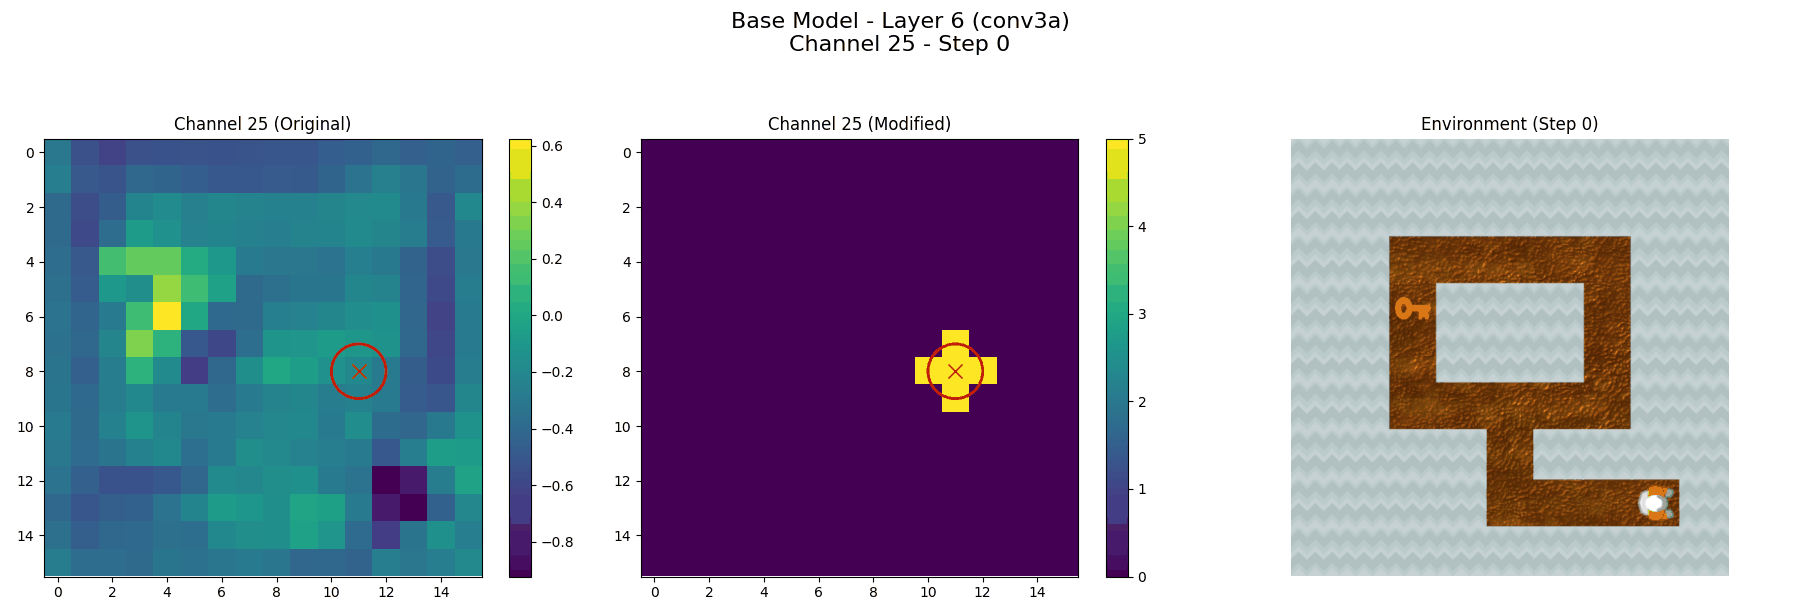
\includegraphics[width=1\textwidth]{figures/intervention_illustration.png}
    \caption{Example of the intervention experiment. We test channels to see the extent to which a single channel is capable of steering the agent to another location given the presence of a single entity in the environment. We consider an intervention a success if the agent enters the modified region. The maze is a 9 by 9 grid, while the conv4a channels have dimensions of 8 by 8, leading to a slightly imperfect mapping.}
    \label{fig:intervention-experiment}
    \end{figure}


    \subsection{Ablation Studies}
    \label{subsec:ablation_studies}
    To systematically assess the role of individual channels, a comprehensive ablation methodology was developed. For each channel in the SAE, episodes were run with only that channel active while ablating all other channels. This allowed measurement of the isolated capability of each channel to support navigation to different entities in the environment. Successful entity collection counts were recorded for each channel across multiple episodes.

    Because the agent has a bias towards randomly walking in a given direction depending on the current policy, it is necessary to rotate the maze so that the direction it's biased towards is the one facing away from the entities. This requires some manual intervention in order to ensure clarity in the results.


    \begin{figure}[h]
        \centering
        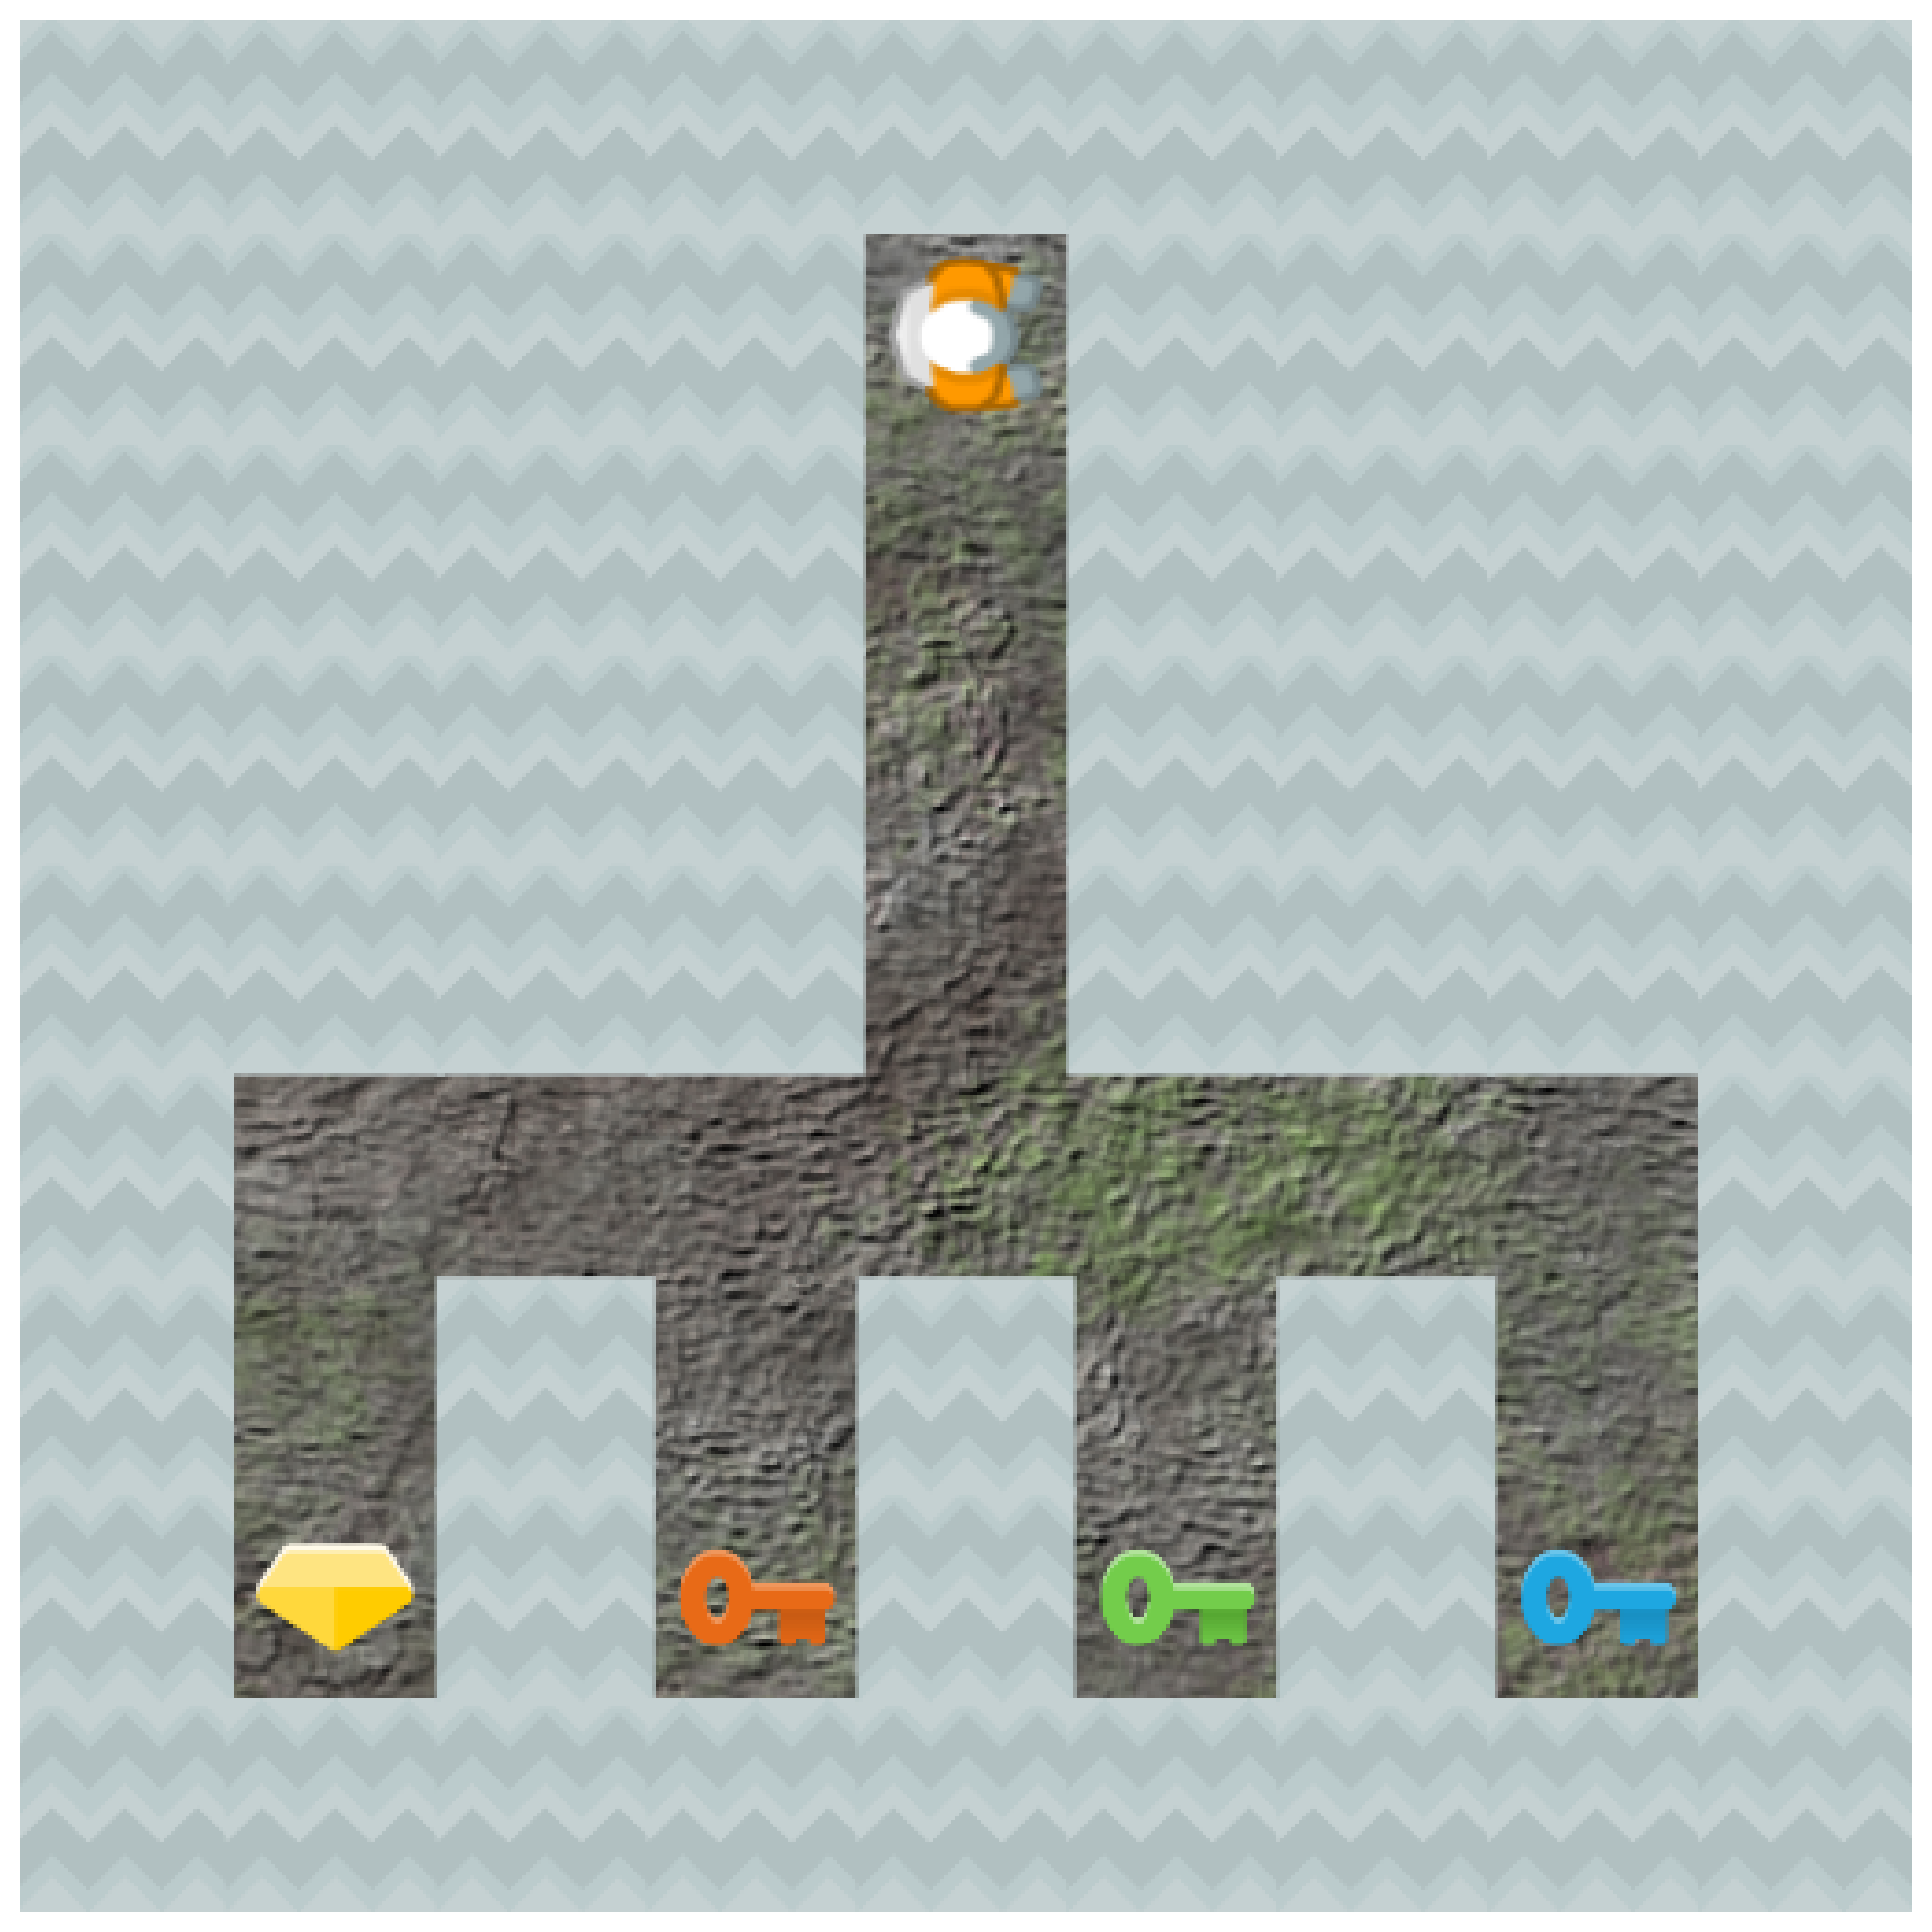
\includegraphics[width=0.8\textwidth]{figures/fork_maze_for_paper.png}
        \caption{The forked maze environment used for steering experiments. The agent starts at the top and must choose between navigating to the original entity (a key, in this case) on the left, or to the artificially targeted region on the right.}
        \label{fig:fork_maze_for_paper}
        \end{figure}

    \

\section{Experimental Design and Evaluation Metrics}


\label{sec:experimental_design_eval}
    \subsection{General Experimental Approach}
    \label{subsec:general_exp_approach}
    The research involved training RL agents and corresponding SAEs, followed by a series of analytical experiments. These experiments included feature visualization to understand learned representations, activation steering and patching to test causal control over agent behavior, and ablation studies to determine the functional importance of individual channels. The primary goal was to dissect how the agent represents and pursues multiple objectives in the Procgen Heist environment and how SAEs might alter or clarify these representations.

    \subsection{Evaluation Metrics}
    \label{subsec:eval_metrics}
    Several metrics were used to evaluate the different components of the research:
    \begin{itemize}
        \item \textbf{For SAE Training (Paper 1):} Performance was primarily tracked using variance explained (aiming for close to 1) and the reward attained on the maze-solving task after SAE integration (>95\% recovery). Sparsity was monitored by examining the number of dead features, the mean number of activating neurons, and the fraction of active neurons (target ~0.001).
        \item \textbf{For Steering and Activation Interventions (Paper 1 \& 2):} Success was measured by the agent's deviation to the artificially targeted zone or behavior change (e.g., moving away from an objective). For scaled-up experiments (Paper 1), the frequency of successful deviation across channels and activation strengths was recorded. For activation patching (Paper 2), the ability to steer the agent predictably was the primary metric.
        \item \textbf{For Ablation Studies (Paper 1):} The key metric was the count of successful entity collections per channel when all other channels were ablated, providing a quantitative measure of each channel's specialization and capability.
        \item \textbf{For Steering Vector Analysis (Paper 2):} The effectiveness of steering vectors was partly assessed by the steerability of different layers (reduction in objective pickups). Channel function was investigated by measuring the frequency with which a channel in an objective steering vector activated most strongly at the location of that particular objective.
    \end{itemize}

    \subsubsection{Intervention experiments}
    When doing our experiments, we would place a specific entity into the environment. We then intervene on a single channel in a single layer by applying a zero mask to the channel setting it to zero and setting a specific region of the channel to a chosen value. In this experiment, we would do a sweep over a range of intervention values between 0 and the maximum values that the channel would reach during typical functioning as determined by sampling from the environment during operation. By running this sweep, we can get a sense of what the different channels do at different intervention strengths. We kept the length of the episode to 20 steps to ensure that the agent would either be able to reach the target zone, or the actual entity, but not both.
    
    For each entity-channel combination, we ran 500 trials with the activation 
    value incrementing linearly: $v_i = i \cdot \frac{v_{\max}}{N}$, where $i$ 
    is the trial index (1 to $N$), $N=500$ is the total number of trials, and 
    $v_{\max}$ is the maximum activation range.
    
    We use a `Q' shaped maze with the design visible in\ref{fig:intervention-experiment} because it was challenging enough that the agent would need to retain its navigational abilities to reach either target, while providing a clear decision point where the agent would need to choose between pursuing the original entity or our artificial target zone. 
    
    We test a single entity at a time in this way meaning that steering that is effective with a particular value on a given channel may not be effective for redirecting the agent in the presence of another entity.
    
    To confirm that our results are robust, we also train SAEs~\cite{bricken2023monosemanticity} on the convolutional layers using techniques from~\cite{gorton_2024_missing} to confirm that the results are not merely the result of polysemanticity.

    \subsection{Channel Ablation Study}
To systematically assess the role of individual channels, we developed a comprehensive ablation methodology. For each channel in the network, we ran episodes with only that channel active while masking all other channels to zero. This allowed us to measure the isolated capability of each channel to support navigation to different entities in the environment. We recorded successful entity collection counts for each channel across  400 rollouts, providing a quantitative measure of each channel's specialization and capability. This methodology allows us identify which channels are sufficient for basic navigation. An example of the maze used is given in \ref{fig:ablation-mazes}.

\begin{figure}[H]
\centering
\begin{minipage}[b]{0.48\textwidth}
    \centering
    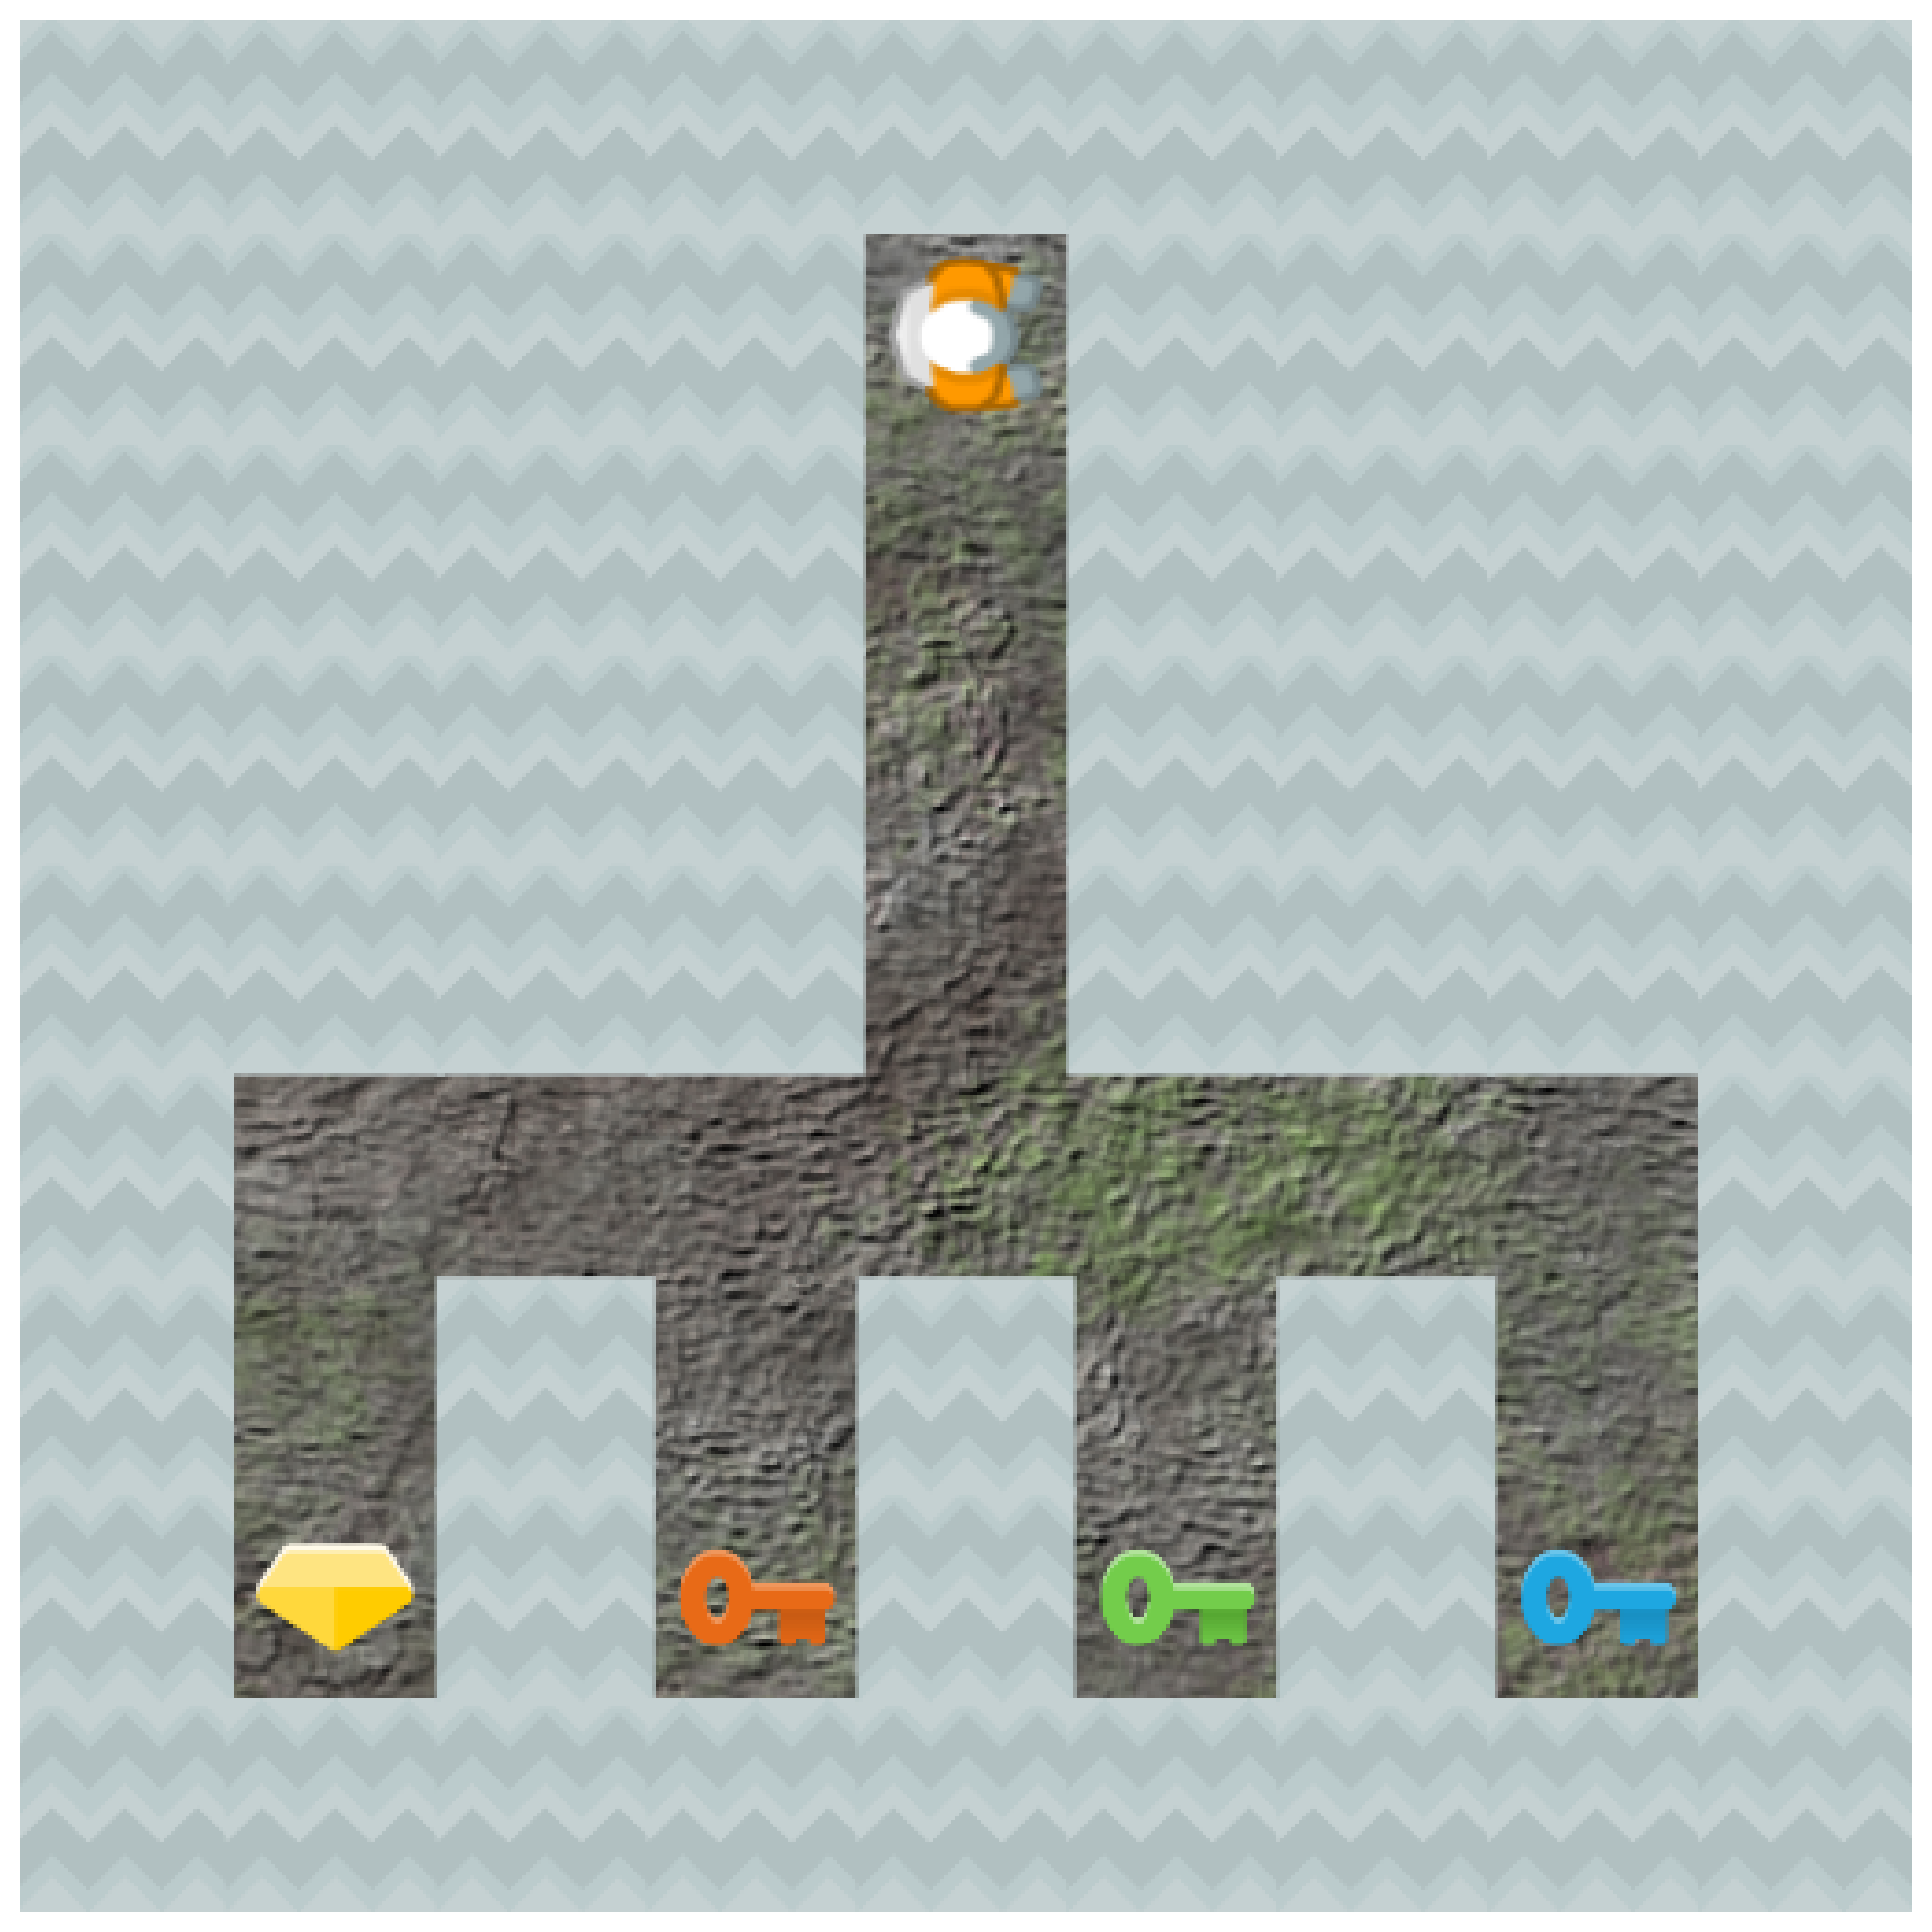
\includegraphics[width=\textwidth]{figures/fork_maze_for_paper.png}
\end{minipage}
\hfill
\begin{minipage}[b]{0.48\textwidth}
    \centering
    % TODO: Add empty_corners_maze_clean.png when available
    \includegraphics[width=\textwidth]{figures/empty_corners_maze_clean.png}
\end{minipage}
\caption{Maze configurations for ablation studies. (a) Fork maze tests individual channel navigation capability by requiring explicit path choices towards different entities and providing sufficient complexity that navigational abilities must be preserved. We orient the stem toward the model's inherent bias direction to minimize false positives. (b) Open maze with entities in corners tests the effect of ablating intervention spans without navigational constraints, ensuring only preferences regarding entity collection are observed.}
\label{fig:ablation-mazes}
\end{figure}
\subsection{Expanded ablation experiments}
To derive further insights from our earlier results, we ablate regions of the network based on their success in modifying model behavior in the previous experiments. Our experiment uses a modified maze which removes all walls, and has the keys and gem randomly distributed in the corners of the maze.

We perform four targeted ablations based on our steering and navigation findings:

\textbf{Ablation 1 (Intervention spans):} We zero out any activations within the value ranges that successfully steered the agent. Specifically, for entity $e$ and channel $c$, we set $h_{c,i,j} = 0$ whenever the activation falls within the successful steering range $\mathcal{S}_{e,c}$ identified in our intervention experiments.

\textbf{Ablation 2 (Navigation channels):} We completely ablate the top 10 channels identified as navigation-critical in our channel isolation study, setting these channels to zero while preserving all others.

\textbf{Ablation 3 (Combined):} We apply both ablations simultaneously, zeroing both the navigation channels and the intervention spans.

\textbf{Ablation 4 (Inverse):} We preserve only the intervention spans that successfully steered the agent in the presence of entity $e$, ablating everything else. This tests whether these spans alone are sufficient for navigation.

\section{Summary}
\label{sec:method_summary_revised}
This chapter detailed the methodologies employed to investigate goal representation and control in a deep reinforcement learning agent. It began with a description of the Procgen Heist environment and the model architectures used. Key interpretability techniques were then outlined, including the training of Sparse Autoencoders, feature visualization methods, the calculation and application of steering vectors for activation interventions, and systematic ablation studies. Finally, the experimental design and the quantitative and qualitative metrics used for evaluation were presented, providing a framework for understanding the results discussed in the subsequent chapter.